\documentclass{article}
\usepackage[top=2in, bottom=1in, left=1in, right=1in]{geometry}
\usepackage{fancyhdr}
\usepackage{amsmath}
\pagestyle{fancyplain}
\usepackage{Sweave}
\begin{document}
\lhead{Math 574M\\ Homework 1}
\rhead{Brian Mannakee\\ \today}
\renewcommand{\vec}[1]{\mathbf{#1}}

\Sconcordance{concordance:Homework1.tex:Homework1.Rnw:%
1 5 1 1 0 12 1}



\begin{enumerate}
  \item X is a continuous random variable with F(X),f(x)
    \begin{enumerate}
      \item \begin{eqnarray*}E(X-a)^2 &=& E[X^2 - 2aX + a^2]\\ &=& E(X^2) -2aE(X) + a^2\end{eqnarray*}
          To minimize, take the first derivative with respect to a and set equal to zero. Then take the second derivative with respect to a and check that the sign is positive.
            \begin{eqnarray*}\frac{d}{da}[E(X^2) - 2aE(X) + a^2] &=& 0 \\ 2E(X) + 2a &=& 0 \\ a &=& E(X)\\
            \frac{d}{da}[2E(X) + 2a] &=& 2 \end{eqnarray*}
            Therefore $a=E(X)$ is a minimum
      \item Set the derivative equal to zero
            \begin{eqnarray*}E(|X-a|) &=& \int|X-a|f(x)dx \\
                                      &=& \int_{-\infty}^a -(X-a)f(x)dx + \int_a^\infty (X-a)f(x)dx \\
                \frac{d}{da}E(|X-a|)  &=& \frac{d}{da}[\int_{-\infty}^a -(X-a)f(x)dx + \int_a^\infty (X-a)f(x)dx] \\
                                    0 &=& \int_{-\infty}^a f(x)dx - \int_a^\infty f(x)dx \\
              \int_{-\infty}^a f(x)dx &=& \int_a^\infty f(x)dx \\
                                      \end{eqnarray*}
            This equality only holds when a is the median of the distribution. In addition $d^2/da^2 = 2f(a) > 0$ so the median is the minimum.
    \end{enumerate}
  \item If $X_1,\dots,X_n$ are i.i.d Bernoulli(p) then $Y = \sum X_i \sim $ Binomial(n,p). If $p \sim beta(\alpha,\beta)$ then their joint pdf is
    \begin{eqnarray*}
        f(y,p) &=& \left[{n \choose y}p^y(1-p)^{n-y}\right] \left[\frac{\Gamma(\alpha + \beta)}{\Gamma(\alpha)\Gamma(
        beta)}p^{\alpha-1}(1-p)^{\beta-1}\right]\\
               &=& {n \choose y}\frac{\Gamma(\alpha + \beta)}{\Gamma(\alpha)\Gamma(\beta)}p^{y+\alpha-1}(1-p)^{n-y+\beta-1}
    \end{eqnarray*}
    We get the marginal of y by integrating out p from the joint distribution.
    \begin{eqnarray*}
      f(y) &=& \int_0^1{n \choose y}\frac{\Gamma(\alpha + \beta)}{\Gamma(\alpha)\Gamma(\beta)}p^{y+\alpha-1}(1-p)^{n-y+\beta-1}dp \\
           &=&{n \choose y}\frac{\Gamma(\alpha + \beta)}{\Gamma(\alpha)\Gamma(\beta)}\int_0^1 p^{y+\alpha-1}(1-p)^{n-y+\beta-1}dp \\
           &=&{n \choose y}\frac{\Gamma(\alpha + \beta)}{\Gamma(\alpha)\Gamma(\beta)}\frac{\Gamma(y+\alpha)\Gamma(n-y+\beta)}{\Gamma(n + \alpha + \beta)}  \text{By definition of the Beta function}
    \end{eqnarray*}
    The posterior $f(p|y)$ is given by the ratio of the joint and the marginal $\frac{f(y,p)}{f(y)}$
    \begin{eqnarray*}
      f(p|y)=\frac{\Gamma(n + \alpha + \beta)}{\Gamma(y+\alpha)\Gamma(n-y+\beta)}p^{y+\alpha-1}(1-p)^{n-y+\beta-1} \sim beta(y+\alpha,n-y+\beta)
    \end{eqnarray*}
      \begin{enumerate}
        \item The posterior mean is the mean of $beta(y+\alpha,n-y+\beta)$ which is
        $$\hat{p}=\frac{y+\alpha}{\alpha + \beta + n}=\frac{\sum_{i=1}^{n}X_i+\alpha}{\alpha + \beta + n}//$$
        \item Decompose MSE = $E(p-\hat{p})^2$ into bias and variance:
         \begin{eqnarray*}
            Var_p(\hat{p}) + Bias_p(\hat{p}) &=& Var_p\left(\frac{\frac{\sum_{i=1}^{n}X_i+\alpha}{\alpha + \beta + n}+\alpha}{\alpha + \beta + n}\right) + \left(E_p\left(\frac{\sum_{i=1}^{n}X_i+\alpha}{\alpha + \beta + n}\right)-p\right)^2\\
                                             &=& \frac{1}{(\alpha + \beta + n)^2}Var_p\left(\sum_{i=1}^{n}X_i\right) + \left(\frac{E_p\left(\sum_{i=1}^{n}X_i\right)+\alpha}{\alpha + \beta + n}-p\right)^2 \\
                                             &=& \frac{np(1-p)}{\alpha + \beta + n)^2} + \left(\frac{np + \alpha}{\alpha + \beta + n} -p\right)^2 \text{because} \sum_{i=1}^{n}X_i\sim \text{binomial(n,p)}
         \end{eqnarray*}
        \item Let $\alpha = \beta = \sqrt{n/4}$ then $$\hat{p}=\frac{\sum_{i=1}^{n}X_i+\sqrt{n/4}}{\sqrt{n/4} + \sqrt{n/4} + n}=\frac{\sum_{i=1}^{n}X_i+\sqrt{n/4}}{\sqrt{n} + n}//$$\\
          \begin{eqnarray*}
            R(p,\hat{p}) &=& \frac{np(1-p)}{\alpha + \beta + n)^2} + \left(\frac{np + \alpha}{\alpha + \beta + n} -p\right)^2 \\
                         &=& \frac{np-np^2}{(\alpha + \beta + n)^2} + \left(\frac{np + \alpha - p\alpha - p\beta - np}{(\alpha + \beta + n)}\right)^2\\
                         &=& \frac{np-np^2}{(\alpha + \beta + n)^2} + \frac{(\alpha - p(\alpha +\beta))^2}{(\alpha + \beta + n)^2}\\
                         &=& \frac{np - np^2 + \alpha^2 - 2p\alpha(\alpha + \beta) + p^2(\alpha + \beta)^2}{(\alpha + \beta + n)^2} \\
                         &=& \frac{np - np^2 + \frac{n}{4} - np + np^2}{(n + \sqrt{n})^2} \\
                         &=& \frac{n}{4(n+\sqrt{n})^2}// \\
          \end{eqnarray*}
      \end{enumerate}
    \item
      \begin{enumerate}
        \item $m(x) = \int_\Theta f(x,\theta) d\theta = \int_\Theta f(x|\theta)\pi(\theta) d\theta$
        \item \begin{eqnarray*}
                r_B(\pi,\hat{\theta}(\vec{X})) &=& \int_\Theta R(\theta,\hat{\theta})\pi(\theta)d\theta \\
                                               &=& \int_\Theta \int_\vec{\mathcal{X}} L(\theta,\hat{\theta}(\vec(X))\pi(\vec{x}|\theta)d\vec{x}\pi(\theta)d\theta \text{ Definition of R()}\\
                                               &=& \int_\Theta \int_\vec{\mathcal{X}} L(\theta,\hat{\theta}(\vec(X))f(\theta,\vec{x})d\vec{x}d\theta \text{      Bayes Rule}\\
                                               &=& \int_\vec{\mathcal{X}} \left[\int_\Theta L(\theta,\hat{\theta}(\vec(X))\pi(\theta|\vec{x})d\theta\right]m(\vec{x})d\vec{x} \text{    Bayes Rule}\\
                                               &=& \int_\vec{\mathcal{X}} r(\hat{\theta}|\vec{x})m(\vec{x})d\vec{x} \text{ Definition of }r(\hat{\theta}|\vec{x}) //\\
              \end{eqnarray*}
        \item The Bayes' Rule $\hat{\theta}(vec{x})$ minimizes the posterior risk $r(\hat{\theta}|\vec{x}) = \int_\Theta L(\theta,\hat{\theta})\pi(\theta|\vec{x})d\theta$, so we take its derivative under squared error loss and set it equal to 0
          \begin{eqnarray*}
            \frac{d}{d\hat{\theta}(\vec{x})}r(\hat{\theta}|\vec{x}) &=& \frac{d}{d\hat{\theta}(\vec{x})}\int_\Theta (\theta-\hat{\theta}(\vec{x})^2\pi(\theta|\vec{x})d\theta \\
                                                                  0 &=& -2\int_\Theta \theta\pi(\theta|\vec{x})d\theta + 2\int_\Theta \hat{\theta}(\vec{x})\pi(\theta|\vec{x})d\theta \\
                      \int_\Theta \theta\pi(\theta|\vec{x})d\theta  &=& \hat{\theta}(\vec{x})\int_\Theta \pi(\theta|\vec{x})d\theta = \hat{\theta}(\vec{x})*1 \\
                                        E(\theta|\vec{X}=\vec{x})   &=& \hat{\theta}(\vec{x}) //
          \end{eqnarray*}
      \end{enumerate}
    \item See prob1.r
    \item
      \begin{enumerate}
        \item Scenario 1 is a balanced classification problem, so the Bayes' boundary can be written as
          $$\left\{\vec{x}:\frac{g_1(\vec{x})}{g_0(\vec{x})}=1\right\}$$
          The two classes are generated by the bivariate normal processes outlined in question 4 giving
           $$ \left\{\vec{x}:\frac{(2\pi)^{-1}\exp\{-\frac{1}{2}[(x_1-2)^2+(x_2-1)^2]\}}{(2\pi)^{-1}\exp\{-\frac{1}{2}[(x_1-1)^2+(x_2-2)^2]\}} = 1 \right\}$$
           $$ \left\{\vec{x}:\frac{(2\pi)^{-1}\exp\{-\frac{1}{2}[x_1^2 - 4x_1 + 4 + x_2^2 -2x_2 + 1]\}}{(2\pi)^{-1}\exp\{-\frac{1}{2}[x_1^2 -2X_1 + 1 + x_2^2 -4x_2 + 4]\}} = 1 \right\}$$
           $$ \left\{\vec{x}:x_1^2 - 4x_1 + 4 + x_2^2 - 2x_2 + 1 = x_1^2 - 2x_1 + 1 + x_2^2 - 4x_2 + 4\right\}$$
           $$ \left\{\vec{x}: x_1 = x_2 \right\}$$
           So the Bayes Rule gives a line with intercept 0 and slope 1, above which points belong to class one and below which they belong to class 0. 
           A plot with the Bayes' Rule line in blue is at the end of this document. The training error for the Bayes Rule is 29\%. 
           The testing error for the Bayes Rule is 22.8\%. 
        \item We can construct the Bayes Rule for Scenario 2 in the same way, although since the means are unknown it can't be simplified meaningfully
          $$ \left\{\vec{x}:\frac{(2\pi)^{-1}\exp\{-\frac{5}{2}[(x_1-\mu_{k1})^2+(x_2-\mu_{k2})^2]\}}{(2\pi)^{-1}\exp\{-\frac{5}{2}[(x_1-\nu_{k1})^2+(x_2-\nu_{k2})^2]\}} = 1 \right\}$$
      \end{enumerate}
    \item 
      \begin{enumerate}
        \item For Scenario 1 the linear estimator derived from the test data is $\hat{C}(\vec{x}) = .5762 + .1606X_1 -.2039X_2$ and we will
        use the decision rule
        $$ \hat{f}(\vec{x}) = \left\{\begin{array}{ll}
                                        1 & \mbox{if $\hat{C}(\vec{x}$) > 0.5} \\
                                        0 & \mbox{if $\hat{C}(\vec{x}$) < 0.5}
                                    \end{array}\right.$$
       A plot with the linear model decision boundary plotted as a blue dashed line is included at the bottom of this document. The training error for the linear model 
       is 25\%, and the testing error is 23.2\% 
        \item For Scenario 2 the linear estimator derived from the test data is $\hat{C}(\vec{x}) = .36129 + .27892X_1 -.06001X_2$ and we will use the same decision rule. 
        The training error for the linear model is 18.5\%, and the testing error is 19\% 
      \end{enumerate}\newpage
    \item[Plots] Blue solid line is the Bayes boundary. Dashed blue lines are the linear model decision boundary. 
\begin{figure}[h]
\begin{center}
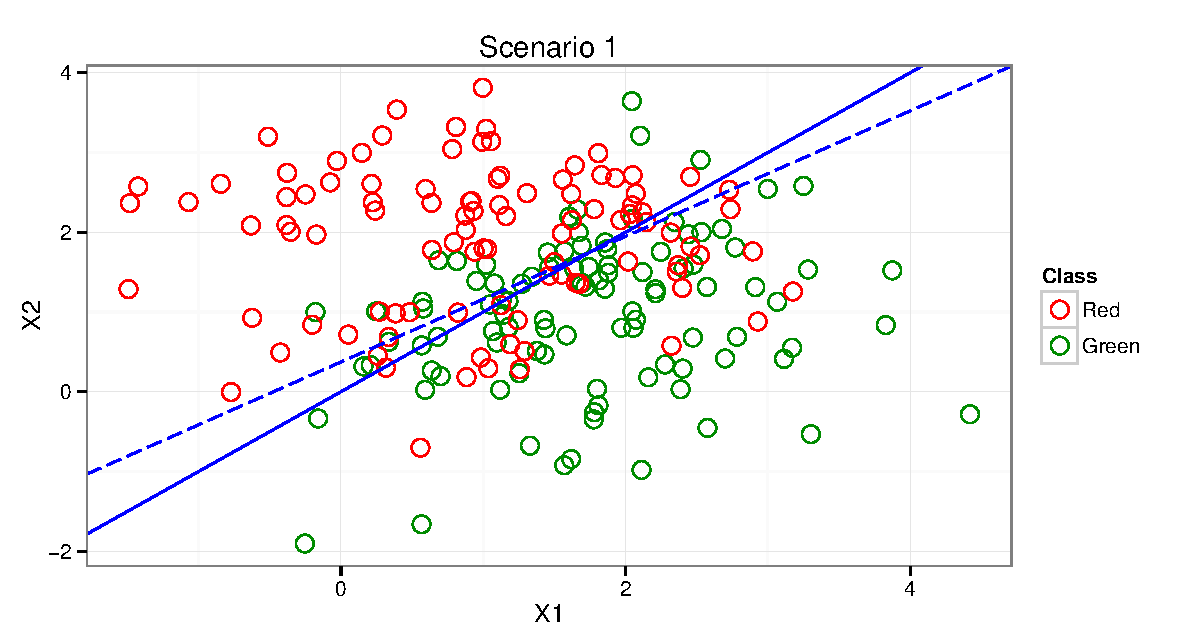
\includegraphics{Homework1-002}
\end{center}
\end{figure} 
\begin{figure}[h]
\begin{center}
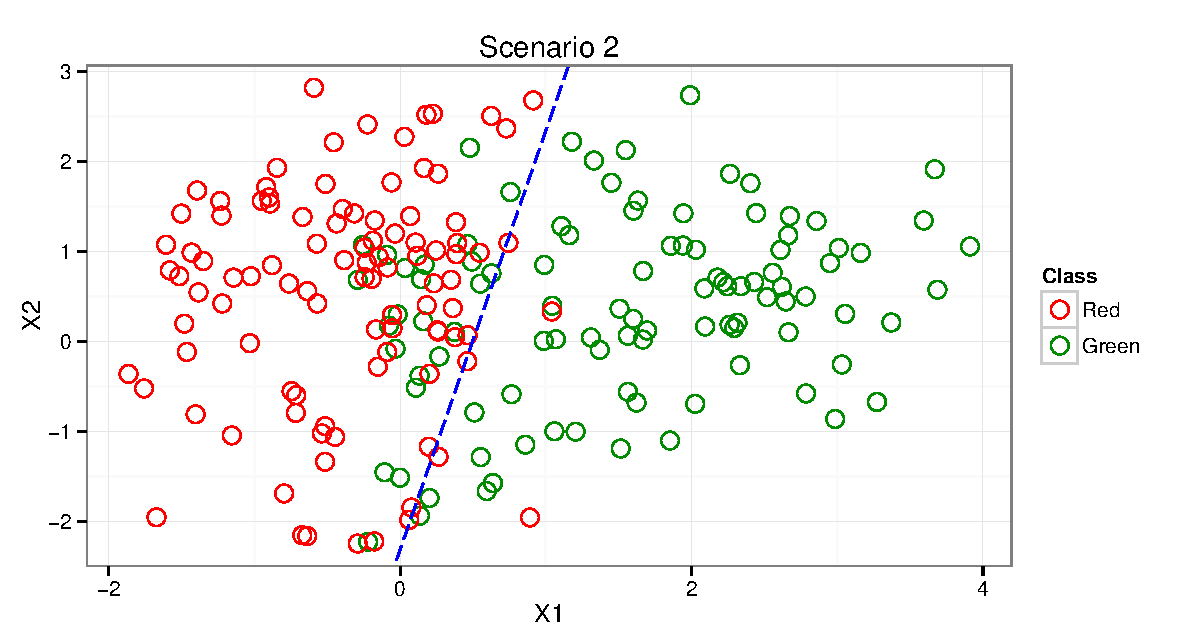
\includegraphics{Homework1-003}
\end{center}
\end{figure} 
\end{enumerate}















\end{document}







